% answers.tex —— 2016 年·天津卷·文科 · 参考答案与详细解析片段
% 由 tools/generate_projects.py 依来源总账自 2016/2016_数学真题_天津文_试题.md + 2016/2016_数学真题_天津文_解析正文.md + 2016/2016_数学真题_天津文_答案要点.md 生成，勿手改（改源 MD 后重跑）


\begin{gktip}
固定原卷不附官方答案。以下为独立推导并经异人盲核对照的解析（非官方答案，等级 D）。第 3 题的截角判定与侧（左）视图朝向、第 13 题行尾数据 \(BE=2AE=2\)、第 14 题解数区间均已按源卷复核；第 17 题图形为示意、不按比例，推演以题设为准。
\end{gktip}

\begin{answer}
\gksolhead{1}{}

\textbf{题目}：

已知集合 \(A=\{1,2,3\}\)，\(B=\{y\mid y=2x-1,x\in A\}\)，则 \(A\cap B=\)（　）

（A）\(\{1,3\}\)　（B）\(\{1,2\}\)　（C）\(\{2,3\}\)　（D）\(\{1,2,3\}\)

\Needspace{4\baselineskip}
\textbf{解析}

由 \(x\in A=\{1,2,3\}\) 得 \(y=2x-1\in\{1,3,5\}\)，即 \(B=\{1,3,5\}\)，故 \(A\cap B=\{1,3\}\)。

\gkanswer{答案：A，\(\{1,3\}\)}

\end{answer}
\begin{answer}
\gksolhead{2}{}

\textbf{题目}：

甲、乙两人下棋，两人下成和棋的概率是 \(\dfrac{1}{2}\)，甲获胜的概率是 \(\dfrac{1}{3}\)，则甲不输的概率为（　）

（A）\(\dfrac{5}{6}\)　（B）\(\dfrac{2}{5}\)　（C）\(\dfrac{1}{6}\)　（D）\(\dfrac{1}{3}\)

\Needspace{4\baselineskip}
\textbf{解析}

“甲不输”即“甲胜或和棋”，两事件互斥，概率为 \(\dfrac{1}{3}+\dfrac{1}{2}=\dfrac{5}{6}\)。（等价算法：乙胜概率为 \(1-\dfrac{1}{2}-\dfrac{1}{3}=\dfrac{1}{6}\)，甲不输概率为 \(1-\dfrac{1}{6}=\dfrac{5}{6}\)。）

\gkanswer{答案：A，\(\dfrac{5}{6}\)}

\end{answer}
\begin{answer}
\gksolhead{3}{}

\textbf{题目}：

将一个长方形沿相邻三个面的对角线截去一个棱锥，得到的几何体的正视图与俯视图如图所示，则该几何体的侧（左）视图为（　）
\nopagebreak[4]
\begin{center}% 第 3 题三视图选择题题图组：2 个已知视图（正视图、俯视图，纵向叠放）+ 4 个选项侧（左）视图（横向排开）。
% 按固定源 PDF 矢量路径换算（1 pt → 0.03515 cm）；原点取图组左下（源页 (67.40, 566.30) pt），y 向上。
% 几何：俯视图为正方形 45.34×45.34 pt，其余为 1:2 竖长方形 45.34×90.67 pt（= 深 × 高）；两已知视图对角线均实线
% （正视图左上→右下、俯视图左下→右上）；选项 (A) 实线、(B) 虚线（均左上→右下），(C) 实线、(D) 虚线（均左下→右上）。
% 全组无尺寸标注；选项字母 (A)–(D) 在各选项图的左下方、图的左边缘之外（不在图下居中）。
\begin{tikzpicture}[line cap=round,line join=round,font=\small,x=0.03515cm,y=0.03515cm]
% ===== 已知视图 =====
% 正视图（竖长方形，实线对角线左上→右下）
\draw (133.30,186.28) rectangle (178.64,276.95);
\draw (133.30,276.95)--(178.64,186.28);
\node[anchor=base west] at (140.22,171.76) {正视图};
% 俯视图（正方形，实线对角线左下→右上）
\draw (133.30,118.27) rectangle (178.64,163.61);
\draw (133.30,118.27)--(178.64,163.61);
\node[anchor=base west] at (140.22,103.82) {俯视图};
% ===== 选项图（四个等大竖长方形，上下边齐平）=====
\draw (19.73,3.23) rectangle (65.07,93.91);
\draw (19.73,93.91)--(65.07,3.23);
\draw (104.30,3.23) rectangle (149.64,93.91);
\draw[dash pattern=on 2.99pt off 2.99pt] (104.30,93.91)--(149.64,3.23);
\draw (189.46,3.23) rectangle (234.79,93.91);
\draw (189.46,3.23)--(234.79,93.91);
\draw (274.90,3.23) rectangle (320.24,93.91);
\draw[dash pattern=on 2.99pt off 2.99pt] (274.90,3.23)--(320.24,93.91);
% 选项字母（图外左下）
\node[anchor=base west] at (0,3.03) {(A)};
\node[anchor=base west] at (85.01,3.03) {(B)};
\node[anchor=base west] at (170.02,3.03) {(C)};
\node[anchor=base west] at (255.02,3.03) {(D)};
\end{tikzpicture}
\end{center}
\nopagebreak[4]
\Needspace{4\baselineskip}
\textbf{解析}

题给正视图为竖长方形（对角线实线、左上→右下），俯视图为正方形（对角线实线、左下→右上）。

\textbf{先定截去的角}。沿相邻三个面的对角线截去的棱锥，其截面三角形的三条边分别落在被截顶点所在的三面上。记长方体 \(a\times b\times h\)，下底面 \(A(0,0,0)\)、\(B(a,0,0)\)、\(C(a,b,0)\)、\(D(0,b,0)\)，上底面对应点加下标 \(1\)。截去前上右角 \(B_{1}(a,0,h)\) 时，截面三角形为 \(BC_{1}A_{1}\)：边 \(A_{1}B\) 在前面（\(y=0\)）上、边 \(BC_{1}\) 在右面（\(x=a\)）上、边 \(A_{1}C_{1}\) 在上面（\(z=h\)）上。正视图沿前后方向投影：\(A_{1}B\) 投为 \(x\) 从 \(0\) 到 \(a\)、\(z\) 从 \(h\) 到 \(0\)，即左上→右下的对角线，且位于可见的前面上，为实线——与题图一致；俯视图沿上下方向投影：\(A_{1}C_{1}\) 投为 \(x\) 从 \(0\) 到 \(a\)、\(y\) 从 \(0\) 到 \(b\)，即左下→右上的对角线，且位于顶面上，为实线——亦与题图一致。对 8 个顶点逐一检验，只有截去前上右角能同时解释给出的两个视图。

\textbf{再看侧（左）视图}。余下几何体的侧视图轮廓为「深 \(\times\) 高」的竖长方形（左端面完整未被截及）。余下 12 条棱中，投影落在外框内部的只有棱 \(BC_{1}\)：\(B\) 在下底面的前右角、\(C_{1}\) 在上底面的后右角，按左视图的投影关系（靠近正视图一侧为物体后方），\(B\) 投在右下方、\(C_{1}\) 投在左上方，即投影为左上→右下方向的对角线；且该棱位于几何体的最右侧面上，从左侧观察时视线被几何体本身遮住，投影应画为虚线。故侧（左）视图为「高矩形加左上→右下虚线对角线」，即选项 (B)。

\gkanswer{答案：B，高矩形与左上→右下虚线对角线的组合}

\end{answer}
\begin{answer}
\gksolhead{4}{}

\textbf{题目}：

已知双曲线 \(\dfrac{x^{2}}{a^{2}}-\dfrac{y^{2}}{b^{2}}=1\)（\(a>0\)，\(b>0\)）的焦距为 \(2\sqrt{5}\)，且双曲线的一条渐近线与直线 \(2x+y=0\) 垂直，则双曲线的方程为（　）

（A）\(\dfrac{x^{2}}{4}-y^{2}=1\)　（B）\(x^{2}-\dfrac{y^{2}}{4}=1\)　（C）\(\dfrac{3x^{2}}{20}-\dfrac{3y^{2}}{5}=1\)　（D）\(\dfrac{3x^{2}}{5}-\dfrac{3y^{2}}{20}=1\)

\Needspace{4\baselineskip}
\textbf{解析}

由焦距 \(2c=2\sqrt{5}\) 得 \(c^{2}=5\)，即 \(a^{2}+b^{2}=5\)。双曲线的渐近线为 \(y=\pm\dfrac{b}{a}x\)，与直线 \(2x+y=0\)（斜率 \(-2\)）垂直，故 \(\dfrac{b}{a}\cdot(-2)=-1\)，即 \(a=2b\)。代入 \(a^{2}+b^{2}=5\) 得 \(5b^{2}=5\)，\(b^{2}=1\)、\(a^{2}=4\)，双曲线方程为 \(\dfrac{x^{2}}{4}-y^{2}=1\)。

\gkanswer{答案：A，\(\dfrac{x^{2}}{4}-y^{2}=1\)}

\end{answer}
\begin{answer}
\gksolhead{5}{}

\textbf{题目}：

设 \(x>0\)，\(y\in\mathbf{R}\)，则“\(x>y\)”是“\(x>|y|\)”的（　）

（A）充要条件　（B）充分而不必要条件

（C）必要而不充分条件　（D）既不充分也不必要条件

\Needspace{4\baselineskip}
\textbf{解析}

必要性：由 \(|y|\geqslant y\) 得 \(x>|y|\geqslant y\)，即 \(x>|y|\Rightarrow x>y\)；不充分性：取 \(x=1\)、\(y=-5\)，有 \(x>y\)，但 \(x<|y|\)。故“\(x>y\)”是“\(x>|y|\)”的必要而不充分条件。

\gkanswer{答案：C，必要而不充分条件}

\end{answer}
\begin{answer}
\gksolhead{6}{}

\textbf{题目}：

已知 \(f(x)\) 是定义在 \(\mathbf{R}\) 上的偶函数，且在区间 \((-\infty,0)\) 上单调递增。若实数 \(a\) 满足 \(f\left(2^{|a-1|}\right)>f\left(-\sqrt{2}\right)\)，则 \(a\) 的取值范围是（　）

（A）\(\left(-\infty,\dfrac{1}{2}\right)\)　（B）\(\left(-\infty,\dfrac{1}{2}\right)\cup\left(\dfrac{3}{2},+\infty\right)\)

（C）\(\left(\dfrac{1}{2},\dfrac{3}{2}\right)\)　（D）\(\left(\dfrac{3}{2},+\infty\right)\)

\Needspace{4\baselineskip}
\textbf{解析}

\Needspace{5\baselineskip}
\(f\) 为偶函数且在 \((-\infty,0)\) 上单调递增，故在 \((0,+\infty)\) 上单调递减，且 \(f(-\sqrt{2})=f(\sqrt{2})\)。由 \(2^{|a-1|}\geqslant 1>0\)、\(\sqrt{2}>0\)，在递减区间上

\nopagebreak[4]
\[
f\left(2^{|a-1|}\right)>f\left(\sqrt{2}\right)\iff 2^{|a-1|}<\sqrt{2}=2^{\frac{1}{2}}\iff |a-1|<\dfrac{1}{2},
\]

解得 \(\dfrac{1}{2}<a<\dfrac{3}{2}\)。

\gkanswer{答案：C，\(\left(\dfrac{1}{2},\dfrac{3}{2}\right)\)}

\end{answer}
\begin{answer}
\gksolhead{7}{}

\textbf{题目}：

已知 \(\triangle ABC\) 是边长为 \(1\) 的等边三角形，点 \(D,E\) 分别是边 \(AB,BC\) 的中点，连接 \(DE\) 并延长到点 \(F\)，使得 \(DE=2EF\)，则 \(\overrightarrow{AF}\cdot\overrightarrow{BC}\) 的值为（　）

（A）\(-\dfrac{8}{5}\)　（B）\(\dfrac{1}{8}\)　（C）\(\dfrac{1}{4}\)　（D）\(\dfrac{11}{8}\)

\Needspace{4\baselineskip}
\textbf{解析}

\Needspace{5\baselineskip}
坐标法：取 \(A(0,0)\)、\(B(1,0)\)、\(C\left(\dfrac{1}{2},\dfrac{\sqrt{3}}{2}\right)\)。\(D\)、\(E\) 分别为 \(AB\)、\(BC\) 的中点：

\nopagebreak[4]
\[
D\left(\dfrac{1}{2},0\right),\qquad E\left(\dfrac{3}{4},\dfrac{\sqrt{3}}{4}\right),\qquad \overrightarrow{DE}=\left(\dfrac{1}{4},\dfrac{\sqrt{3}}{4}\right).
\]

\Needspace{5\baselineskip}
由 \(DE=2EF\) 且 \(F\) 在 \(DE\) 的延长线上，\(\overrightarrow{EF}=\dfrac{1}{2}\overrightarrow{DE}=\left(\dfrac{1}{8},\dfrac{\sqrt{3}}{8}\right)\)，故 \(F=\left(\dfrac{7}{8},\dfrac{3\sqrt{3}}{8}\right)\)。于是

\nopagebreak[4]
\[
\overrightarrow{AF}\cdot\overrightarrow{BC}=\left(\dfrac{7}{8},\dfrac{3\sqrt{3}}{8}\right)\cdot\left(-\dfrac{1}{2},\dfrac{\sqrt{3}}{2}\right)=-\dfrac{7}{16}+\dfrac{9}{16}=\dfrac{1}{8}.
\]

\gkanswer{答案：B，\(\dfrac{1}{8}\)}

\end{answer}
\begin{answer}
\gksolhead{8}{}

\textbf{题目}：

已知函数 \(f(x)=\sin^{2}\dfrac{\omega x}{2}+\dfrac{1}{2}\sin\omega x-\dfrac{1}{2}\)（\(\omega>0\)），\(x\in\mathbf{R}\)。若 \(f(x)\) 在区间 \((\pi,2\pi)\) 内没有零点，则 \(\omega\) 的取值范围是（　）

（A）\(\left(0,\dfrac{1}{8}\right]\)　（B）\(\left(0,\dfrac{1}{4}\right]\cup\left[\dfrac{5}{8},1\right)\)

（C）\(\left(0,\dfrac{5}{8}\right]\)　（D）\(\left(0,\dfrac{1}{8}\right]\cup\left[\dfrac{1}{4},\dfrac{5}{8}\right]\)

\Needspace{4\baselineskip}
\textbf{解析}

\Needspace{5\baselineskip}
降幂：\(\sin^{2}\dfrac{\omega x}{2}=\dfrac{1-\cos\omega x}{2}\)，故

\nopagebreak[4]
\[
f(x)=\dfrac{1-\cos\omega x}{2}+\dfrac{1}{2}\sin\omega x-\dfrac{1}{2}=\dfrac{1}{2}\left(\sin\omega x-\cos\omega x\right)=\dfrac{\sqrt{2}}{2}\sin\left(\omega x-\dfrac{\pi}{4}\right).
\]

零点满足 \(\omega x-\dfrac{\pi}{4}=k\pi\)（\(k\in\mathbf{Z}\)），即 \(x=\dfrac{(4k+1)\pi}{4\omega}\)。\(f\) 在 \((\pi,2\pi)\) 内没有零点，等价于不存在整数 \(k\) 使 \(4\omega<4k+1<8\omega\)（端点允许取到）。

若 \(\omega\geqslant 1\)，区间 \((4\omega,8\omega)\) 的长度为 \(4\omega\geqslant 4\) 且左端点是 \(4\) 的倍数，该开区间必含一个 \(\equiv 1\pmod 4\) 的整数，不合；若 \(0<\omega<1\)，则 \(8\omega<8\)，候选只有 \(4k+1\in\{1,5\}\)：\(1\in(4\omega,8\omega)\iff\dfrac{1}{8}<\omega<\dfrac{1}{4}\)，\(5\in(4\omega,8\omega)\iff\dfrac{5}{8}<\omega<1\)，两区间均须排除。

故 \(\omega\in\left(0,\dfrac{1}{8}\right]\cup\left[\dfrac{1}{4},\dfrac{5}{8}\right]\)（端点核验：\(\omega=\dfrac{1}{8}\)、\(\dfrac{5}{8}\) 时零点含 \(x=2\pi\)，\(\omega=\dfrac{1}{4}\) 时零点含 \(x=\pi\)，均落在开区间端点，允许）。

\gkanswer{答案：D，\(\left(0,\dfrac{1}{8}\right]\cup\left[\dfrac{1}{4},\dfrac{5}{8}\right]\)}

\end{answer}
\begin{answer}
\gksolhead{9}{}

\textbf{题目}：

\(\mathrm{i}\) 是虚数单位，复数 \(z\) 满足 \((1+\mathrm{i})z=2\)，则 \(z\) 的实部为 \(\underline{\qquad}\)。

\Needspace{4\baselineskip}
\textbf{解析}

\Needspace{5\baselineskip}
由 \((1+\mathrm{i})z=2\) 得

\nopagebreak[4]
\[
z=\dfrac{2}{1+\mathrm{i}}=\dfrac{2(1-\mathrm{i})}{(1+\mathrm{i})(1-\mathrm{i})}=1-\mathrm{i},
\]

实部为 \(1\)。

\gkanswer{答案：\(1\)}

\end{answer}
\begin{answer}
\gksolhead{10}{}

\textbf{题目}：

已知函数 \(f(x)=(2x+1)\mathrm{e}^{x}\)，\(f'(x)\) 为 \(f(x)\) 的导函数，则 \(f'(0)\) 的值为 \(\underline{\qquad}\)。

\Needspace{4\baselineskip}
\textbf{解析}

\(f'(x)=2\mathrm{e}^{x}+(2x+1)\mathrm{e}^{x}=(2x+3)\mathrm{e}^{x}\)，故 \(f'(0)=3\)。

\gkanswer{答案：\(3\)}

\end{answer}
\begin{answer}
\gksolhead{11}{}

\textbf{题目}：

阅读如下的程序框图，运行相应的程序，则输出 \(S\) 的值为 \(\underline{\qquad}\)。
\nopagebreak[4]
\begin{center}% 第 11 题程序框图（累减计数型，双菱形双汇入结构）：与同省理卷第 4 题为同一矢量图（纯平移 Δx=+371.68、Δy=-7.15 pt，
% 固定源两卷各自核验），按固定源 PDF 逐框重绘（10 框；1 pt → 0.04 cm）。
% 结构要点（易错，矢量路径逐段核对）：
%   主干 x=0（两个菱形与主线上全部处理框同一中心线）；左支 x=-2.45（S=2S）；右回线 x=+2.34。
%   第一菱形「否」自左顶点向左折下入 S=2S，其回接自框底垂直下、水平右，汇入主干 y=4.87
%   （S=S-6 之后、n=n+1 之前）；第二菱形「否」自右顶点向右、向上至 y=7.45、向左汇入主干
%   （n=1 之后、第一菱形之前）。两处汇入高度不同，均不做自环。
%   全图 11 个箭头；输出框为向右倾平行四边形；无输入框。
\begin{tikzpicture}[>=stealth,every node/.style={font=\small},
  term/.style={draw,rounded corners,minimum width=1.5cm,minimum height=5.5mm},
  box/.style={draw,minimum height=5.5mm,inner xsep=4pt},
  io/.style={draw,trapezium,trapezium left angle=70,trapezium right angle=110,minimum width=1.8cm,minimum height=5.5mm},
  decision/.style={draw,diamond,aspect=4,minimum width=3.2cm,inner sep=0pt}]
\node[term] (start) at (0,10.36) {开始};
\node[box] (s4) at (0,9.16) {\(S=4\)};
\node[box] (n1) at (0,8.02) {\(n=1\)};
\node[decision] (t1) at (0,6.75) {\(S\geqslant 6?\)};
\node[box] (s6) at (0,5.46) {\(S=S-6\)};
\node[box] (s2s) at (-2.45,5.46) {\(S=2S\)};
\node[box] (np1) at (0,4.28) {\(n=n+1\)};
\node[decision] (t2) at (0,3.03) {\(n>3?\)};
\node[io] (out) at (0,1.74) {输出 \(S\)};
\node[term] (end) at (0,0.46) {结束};
\draw[->] (start)--(s4);
\draw[->] (s4)--(n1);
\draw[->] (n1)--(t1);
\draw[->] (t1.south)--(s6.north);
\draw[->] (s6)--(np1);
\draw[->] (np1)--(t2);
\draw[->] (t2.south)--(out.north);
\draw[->] (out)--(end);
% 第一菱形「否」：左顶点向左折下入 S=2S
\draw[->] (t1.west) -| (s2s.north);
% S=2S 回接：框底垂直向下、水平向右汇入主干（汇入点高于 n=n+1）
\draw[->] (s2s.south) |- (0,4.87);
% 第二菱形「否」：右顶点向右、向上、向左汇入主干（汇入点高于第一菱形）
\draw[->] (t2.east) -- (2.34,3.03) -- (2.34,7.45) -- (0,7.45);
% 分支标注（「否」在各自水平线上方、「是」在主干竖线右侧）
\node at (-1.64,7.05) {否};
\node at (0.65,6.15) {是};
\node at (1.55,3.38) {否};
\node at (0.65,2.42) {是};
\end{tikzpicture}
\end{center}
\nopagebreak[4]
\Needspace{4\baselineskip}
\textbf{解析}

按框图逐步执行（先判断 \(S\geqslant 6?\)：否则执行 \(S=2S\)，是则执行 \(S=S-6\)；再 \(n=n+1\)，判断 \(n>3?\)：否则回到 \(S\geqslant 6?\)，是则输出）：

\begin{itemize}
\item \((S,n)=(4,1)\)：\(4\geqslant 6\) 不成立，\(S=2S=8\)，\(n=2\)；\(2>3\) 不成立；
\item \((S,n)=(8,2)\)：\(8\geqslant 6\) 成立，\(S=8-6=2\)，\(n=3\)；\(3>3\) 不成立；
\item \((S,n)=(2,3)\)：\(2\geqslant 6\) 不成立，\(S=2S=4\)，\(n=4\)；\(4>3\) 成立，输出 \(S=4\)。
\end{itemize}

\gkanswer{答案：\(4\)}

\end{answer}
\begin{answer}
\gksolhead{12}{}

\textbf{题目}：

已知圆 \(C\) 的圆心在 \(x\) 轴的正半轴上，点 \(M(0,\sqrt{5})\) 在圆 \(C\) 上，且圆心到直线 \(2x-y=0\) 的距离为 \(\dfrac{4\sqrt{5}}{5}\)，则圆 \(C\) 的方程为 \(\underline{\qquad}\)。

\Needspace{4\baselineskip}
\textbf{解析}

\Needspace{5\baselineskip}
设圆心 \(C(a,0)\)（\(a>0\)）、半径为 \(r\)。由 \(M(0,\sqrt{5})\) 在圆上得 \(r^{2}=a^{2}+5\)；由圆心到直线 \(2x-y=0\) 的距离为 \(\dfrac{4\sqrt{5}}{5}\)：

\nopagebreak[4]
\[
\dfrac{|2a-0|}{\sqrt{2^{2}+(-1)^{2}}}=\dfrac{2a}{\sqrt{5}}=\dfrac{4\sqrt{5}}{5},
\]

解得 \(a=2\)，\(r^{2}=4+5=9\)。故圆 \(C\) 的方程为 \((x-2)^{2}+y^{2}=9\)。

\gkanswer{答案：\((x-2)^{2}+y^{2}=9\)}

\end{answer}
\begin{answer}
\gksolhead{13}{}

\textbf{题目}：

如图，\(AB\) 是圆的直径，弦 \(CD\) 与 \(AB\) 相交于点 \(E\)，\(BE=2AE=2\)，\(BD=ED\)，则线段 \(CE\) 的长为 \(\underline{\qquad}\)。
\nopagebreak[4]
\begin{center}% 第 13 题圆：与同省理卷第 12 题为同一矢量图（圆心横坐标 594.74 与半径 40.08 pt 两卷相同，仅纵向平移 122.77 pt；
% 固定源两卷各自核验），按固定源 PDF 矢量路径换算（1 pt → 0.03515 cm），取圆心为原点、y 向上。
% 圆心半径同上；直径 AB 水平过圆心；弦 CD 自左上（C 在圆上）经 E（在 AB 上）至右下（D 在圆上，BD=ED）；
% 线段 BD。图中不标圆心、无直角标记、无长度数字。
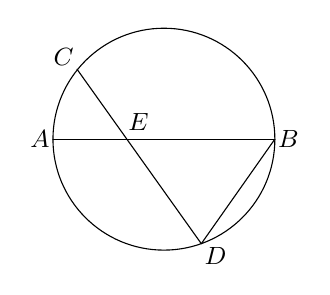
\begin{tikzpicture}[line cap=round,line join=round,font=\small]
\draw (0,0) circle (1.409);
\draw (-1.409,0)--(1.409,0);
\draw (-1.103,0.888)--(0.475,-1.327);
\draw (1.409,0)--(0.475,-1.327);
\node[above left,inner sep=1pt] at (-1.103,0.888) {$C$};
\node[left,inner sep=1pt] at (-1.409,0) {$A$};
\node at (-0.324,0.220) {$E$};
\node[right,inner sep=1pt] at (1.409,0) {$B$};
\node[below right,inner sep=1pt] at (0.475,-1.327) {$D$};
\end{tikzpicture}
\end{center}
\nopagebreak[4]
\Needspace{4\baselineskip}
\textbf{解析}

由 \(BE=2AE=2\) 得 \(AE=1\)、\(BE=2\)，故 \(AB=3\)、圆的半径 \(R=\dfrac{3}{2}\)。以圆心为原点、\(AB\) 所在直线为 \(x\) 轴：\(A\left(-\dfrac{3}{2},0\right)\)、\(B\left(\dfrac{3}{2},0\right)\)、\(E\left(-\dfrac{1}{2},0\right)\)。

\Needspace{5\baselineskip}
由 \(BD=ED\)，点 \(D\) 在线段 \(EB\) 的垂直平分线 \(x=\dfrac{1}{2}\) 上；又 \(D\) 在圆上：\(\left(\dfrac{1}{2}\right)^{2}+y_{D}^{2}=\left(\dfrac{3}{2}\right)^{2}\)，得 \(|y_{D}|=\sqrt{2}\)，故

\nopagebreak[4]
\[
ED=\sqrt{\left(\dfrac{1}{2}+\dfrac{1}{2}\right)^{2}+(\sqrt{2})^{2}}=\sqrt{3}.
\]

由相交弦定理（\(E\) 为弦 \(AB\) 与弦 \(CD\) 的交点）：\(EA\cdot EB=EC\cdot ED\)，即 \(1\times 2=EC\times\sqrt{3}\)，故 \(CE=\dfrac{2}{\sqrt{3}}=\dfrac{2\sqrt{3}}{3}\)。

\gkanswer{答案：\(\dfrac{2\sqrt{3}}{3}\)}

\end{answer}
\begin{answer}
\gksolhead{14}{}

\textbf{题目}：

\Needspace{5\baselineskip}
已知函数

\nopagebreak[4]
\[
f(x)=\begin{cases}
x^{2}+(4a-3)x+3a, & x<0,\\
\log_{a}(x+1)+1, & x\geqslant 0,
\end{cases}
\]

（\(a>0\) 且 \(a\neq 1\)）在 \(\mathbf{R}\) 上单调递减，且关于 \(x\) 的方程 \(|f(x)|=2-\dfrac{x}{3}\) 恰有两个不相等的实数解，则 \(a\) 的取值范围是 \(\underline{\qquad}\)。

\Needspace{4\baselineskip}
\textbf{解析}

由单调递减先定 \(a\) 的范围：\(x<0\) 时 \(f(x)=x^{2}+(4a-3)x+3a\) 递减，需其顶点横坐标 \(\dfrac{3-4a}{2}\geqslant 0\)，即 \(a\leqslant\dfrac{3}{4}\)；\(x\geqslant 0\) 时 \(\log_{a}(x+1)+1\) 递减，需 \(0<a<1\)；接合处需 \(f(0^{-})=3a\geqslant f(0)=1\)，即 \(a\geqslant\dfrac{1}{3}\)。故 \(a\in\left[\dfrac{1}{3},\dfrac{3}{4}\right]\)。记 \(x^{*}=\dfrac{1}{a}-1\in\left[\dfrac{1}{3},2\right]\)（即 \(f(x^{*})=0\)），在此范围内分别数两支的解：

\Needspace{5\baselineskip}
\textbf{\(x<0\) 支}：\(f\) 在 \((-\infty,0)\) 上递减，且 \(f(x)>f(0^{-})=3a>0\)，故 \(|f(x)|=f(x)\)，方程化为

\nopagebreak[4]
\[
x^{2}+(4a-3)x+3a=2-\dfrac{x}{3},\quad\text{即}\quad x^{2}+\left(4a-\dfrac{8}{3}\right)x+(3a-2)=0,
\]

两根之积为 \(3a-2\)，判别式 \(\Delta=16\left(a-\dfrac{2}{3}\right)\left(a-\dfrac{17}{12}\right)\)。

\begin{itemize}
\item \(a<\dfrac{2}{3}\) 时 \(3a-2<0\)，两根异号，恰有 \(1\) 个负根；
\item \(a=\dfrac{2}{3}\) 时方程即 \(x^{2}=0\)，重根 \(x=0\) 不在 \(x<0\) 内，\(0\) 个负根；
\item \(\dfrac{2}{3}<a\leqslant\dfrac{3}{4}<\dfrac{17}{12}\) 时 \(\Delta<0\)，无实根，\(0\) 个负根。
\end{itemize}

\Needspace{5\baselineskip}
\textbf{\(x\geqslant 0\) 支}：恒恰有 \(1\) 解。在 \([0,x^{*}]\) 上 \(|f(x)|=f(x)\leqslant f(0)=1\)，而 \(2-\dfrac{x}{3}\geqslant 2-\dfrac{x^{*}}{3}\geqslant\dfrac{4}{3}>1\)，无解；在 \((x^{*},+\infty)\) 上方程即

\nopagebreak[4]
\[
\psi(x)=-\log_{a}(x+1)+\dfrac{x}{3}-3=0,
\]

\(\psi'(x)=\dfrac{1}{(x+1)|\ln a|}+\dfrac{1}{3}>0\)，\(\psi\) 严格递增，且 \(\psi(x^{*})=\dfrac{x^{*}}{3}-2<0\)、\(x\to+\infty\) 时 \(\psi\to+\infty\)，故恰有 \(1\) 解。

\textbf{合计}：恰有两个不相等的实数解 \(\iff\) 负侧恰有 \(1\) 解 \(\iff a\in\left[\dfrac{1}{3},\dfrac{2}{3}\right)\)。（数值抽验：\(a=0.6\) 时两根约为 \(-0.333\) 与 \(2.19\)，恰 2 解；\(a=\dfrac{2}{3}\) 与 \(a=0.7\) 均仅 1 解。）

\gkanswer{答案：\(\left[\dfrac{1}{3},\dfrac{2}{3}\right)\)}

\end{answer}
\begin{answer}
\gksolhead{15}{}

\textbf{题目}：

在 \(\triangle ABC\) 中，内角 \(A,B,C\) 所对应的边分别为 \(a,b,c\)。已知 \(a\sin 2B=\sqrt{3}b\sin A\)。

（1） 求 \(B\)；

（2） 若 \(\cos A=\dfrac{1}{3}\)，求 \(\sin C\) 的值。

\Needspace{4\baselineskip}
\textbf{解析}

\gksubpart{(1)}

\Needspace{5\baselineskip}
由正弦定理 \(a=2R\sin A\)、\(b=2R\sin B\) 代入 \(a\sin 2B=\sqrt{3}b\sin A\)：

\nopagebreak[4]
\[
2R\sin A\cdot 2\sin B\cos B=\sqrt{3}\cdot 2R\sin B\sin A,
\]

约去 \(2R\sin A\sin B\neq 0\) 得 \(2\cos B=\sqrt{3}\)，\(\cos B=\dfrac{\sqrt{3}}{2}\)。因 \(0<B<\pi\)，故 \(B=\dfrac{\pi}{6}\)。

\gksubpart{(2)}

\Needspace{5\baselineskip}
由 \(\cos A=\dfrac{1}{3}\)、\(0<A<\pi\) 得 \(\sin A=\sqrt{1-\dfrac{1}{9}}=\dfrac{2\sqrt{2}}{3}\)。\(C=\pi-A-B=\dfrac{5\pi}{6}-A\)，故

\nopagebreak[4]
\[
\sin C=\sin\dfrac{5\pi}{6}\cos A-\cos\dfrac{5\pi}{6}\sin A=\dfrac{1}{2}\cdot\dfrac{1}{3}-\left(-\dfrac{\sqrt{3}}{2}\right)\cdot\dfrac{2\sqrt{2}}{3}=\dfrac{1}{6}+\dfrac{\sqrt{6}}{3}=\dfrac{1+2\sqrt{6}}{6}.
\]

\gkanswer{答案（1）：\(B=\dfrac{\pi}{6}\)。}

\gkanswer{答案（2）：\(\sin C=\dfrac{1+2\sqrt{6}}{6}\)。}

\end{answer}
\begin{answer}
\gksolhead{16}{}

\textbf{题目}：

某化肥厂生产甲、乙两种混合肥料，需要 \(A,B,C\) 三种主要原料。生产 \(1\) 车皮甲种肥料和生产 \(1\) 车皮乙种肥料所需三种原料的吨数如下表所示：
\nopagebreak[4]
\begin{center}% 第 16 题原料用量表：按固定源 PDF 矢量路径换算（1 pt → 0.03515 cm）；原点取表格左下（源页 (913.89, 512.81) pt），y 向上。
% 4 条横线（含上下外框）、5 条竖线；表头行高 30.63 pt 约为数据行 15.51 pt 的两倍；
% 角格 45° 斜线自左上至右下，右上「原料」（对应 A,B,C 三列）、左下「肥料」（对应甲、乙两行）。
% 列宽（自左至右）66.28 / 20.22 / 20.84 / 22.85 pt；列标 A,B,C 为数学斜体，数据 4/8/3/5/5/10 为正体数字。
\begin{tikzpicture}[line cap=round,line join=round,font=\small,x=0.03515cm,y=0.03515cm]
% 横线（4 条）
\draw (0,61.65)--(130.59,61.65);
\draw (0,31.02)--(130.59,31.02);
\draw (0,15.51)--(130.59,15.51);
\draw (0,0)--(130.59,0);
% 竖线（5 条）
\draw (0.20,0)--(0.20,61.65);
\draw (66.48,0)--(66.48,61.65);
\draw (86.70,0)--(86.70,61.65);
\draw (107.54,0)--(107.54,61.65);
\draw (130.39,0)--(130.39,61.65);
% 角格斜线（左上→右下）
\draw (0.40,61.45)--(66.29,31.22);
% 斜线表头两角文字
\node[anchor=base west] at (39.32,50.87) {原料};
\node[anchor=base west] at (6.38,35.76) {肥料};
% 表头列标与数据行（各列居中）
\node[anchor=base] at (76.59,43.71) {\(A\)};
\node[anchor=base] at (97.12,43.71) {\(B\)};
\node[anchor=base] at (118.97,43.71) {\(C\)};
\node[anchor=base] at (33.34,20.24) {甲};
\node[anchor=base] at (76.59,20.24) {\(4\)};
\node[anchor=base] at (97.12,20.24) {\(8\)};
\node[anchor=base] at (118.97,20.24) {\(3\)};
\node[anchor=base] at (33.34,4.73) {乙};
\node[anchor=base] at (76.59,4.73) {\(5\)};
\node[anchor=base] at (97.12,4.73) {\(5\)};
\node[anchor=base] at (118.97,4.73) {\(10\)};
\end{tikzpicture}
\end{center}
\nopagebreak[4]
现有 \(A\) 种原料 \(200\) 吨，\(B\) 种原料 \(360\) 吨，\(C\) 种原料 \(300\) 吨，在此基础上生产甲乙两种肥料。已知生产 \(1\) 车皮甲种肥料，产生的利润为 \(2\) 万元；生产 \(1\) 车皮乙种肥料，产生的利润为 \(3\) 万元。分别用 \(x\)、\(y\) 表示生产甲、乙两种肥料的车皮数。

（1） 用 \(x,y\) 列出满足生产条件的数学关系式，并画出相应的平面区域；

（2） 问分别生产甲、乙两种肥料各多少车皮，能够产生最大的利润？并求出此最大利润。

\Needspace{4\baselineskip}
\textbf{解析}

\gksubpart{(1)}

设生产甲 \(x\) 车皮、乙 \(y\) 车皮。由表，三种原料的约束为 \(4x+5y\leqslant 200\)、\(8x+5y\leqslant 360\)、\(3x+10y\leqslant 300\)，且 \(x\geqslant 0\)、\(y\geqslant 0\)。平面区域为该不等式组的解集，是以 \(O(0,0)\)、\(R(45,0)\)、\(M(40,8)\)、\(P(20,24)\)、\(Q(0,30)\) 为顶点的五边形区域（\(M\) 为 \(4x+5y=200\) 与 \(8x+5y=360\) 的交点，\(P\) 为 \(4x+5y=200\) 与 \(3x+10y=300\) 的交点）。

\gksubpart{(2)}

目标函数 \(z=2x+3y\) 为线性函数，最大值在可行域顶点取得。各顶点处：\(z(O)=0\)、\(z(R)=90\)、\(z(M)=104\)、\(z(P)=112\)、\(z(Q)=90\)。故当 \(x=20\)、\(y=24\) 时利润最大，即生产甲种肥料 \(20\) 车皮、乙种肥料 \(24\) 车皮，最大利润为 \(2\times 20+3\times 24=112\) 万元。（校验：此时 \(A\) 种原料 \(4\times 20+5\times 24=200\) 恰好用完、\(C\) 种 \(3\times 20+10\times 24=300\) 恰好用完、\(B\) 种 \(8\times 20+5\times 24=280\leqslant 360\)。）

\gkanswer{答案（1）：\(4x+5y\leqslant 200\)，\(8x+5y\leqslant 360\)，\(3x+10y\leqslant 300\)，\(x\geqslant 0\)，\(y\geqslant 0\)；平面区域为该不等式组的解集（以 \((0,0)\)、\((45,0)\)、\((40,8)\)、\((20,24)\)、\((0,30)\) 为顶点的五边形区域）。}

\gkanswer{答案（2）：甲 \(20\) 车皮、乙 \(24\) 车皮，最大利润 \(112\) 万元。}

\end{answer}
\begin{answer}
\gksolhead{17}{}

\textbf{题目}：

如图，四边形 \(ABCD\) 是平行四边形，平面 \(AED\perp\) 平面 \(ABCD\)，\(EF\parallel AB\)，\(AB=2\)，\(BC=EF=1\)，\(AE=\sqrt{6}\)，\(DE=3\)，\(\angle BAD=60^{\circ}\)，\(G\) 为 \(BC\) 的中点。
\nopagebreak[4]
\begin{center}% 第 17 题多面体（平行四边形 ABCD 上立平面 AED，含 F、E 与 BC 中点 G）：
% 按固定源 PDF 矢量路径端点换算（1 pt → 0.03515 cm）；原点取 C 点，y 向上。
% 源页顶点 pt：E(391.63,174.74)、F(334.74,174.74)、A(344.37,320.41)、B(230.60,320.41)、
% C(184.85,337.27)、D(298.62,337.27)、G(207.73,328.84)（G 为 BC 中点，坐标精确吻合）。
% 实线 6 条：EF、FC、CD、DA、DE、AE；虚线 6 条：CB、BA、BD、GF、BF、BE。先画虚线后画实线。
% 注：该图为示意，不按题设比例（∠BAD 实测约 20°、AB:BC 实测约 2.33:1），照源描摹，不按数值重定比例。
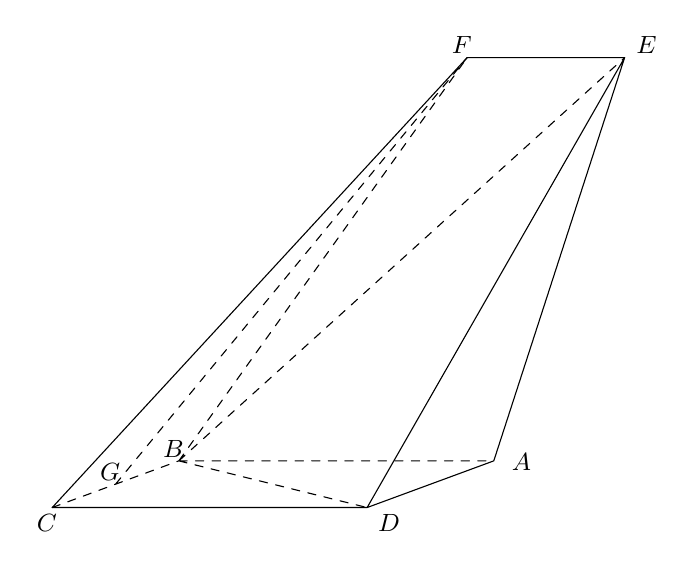
\begin{tikzpicture}[line cap=round,line join=round,font=\small,x=0.03515cm,y=0.03515cm]
\coordinate (E) at (206.78,162.53);
\coordinate (F) at (149.89,162.53);
\coordinate (A) at (159.52,16.86);
\coordinate (B) at (45.75,16.86);
\coordinate (C) at (0,0);
\coordinate (D) at (113.77,0);
\coordinate (G) at (22.88,8.43);
% 虚线先画
\draw[dashed] (C)--(B) (B)--(A) (B)--(D) (G)--(F) (B)--(F) (B)--(E);
% 实线后画
\draw (E)--(F) (F)--(C) (C)--(D) (D)--(A) (D)--(E) (A)--(E);
% 标注（显式坐标：源字形左端与基线换算；不并入线段）
\node[anchor=base west] at (140.86,163.87) {$F$};
\node[anchor=base west] at (207.53,163.87) {$E$};
\node[anchor=base west] at (162.56,13.27) {$A$};
\node[anchor=base west] at (36.58,18.20) {$B$};
\node[anchor=base west] at (13.82,9.77) {$G$};
\node[anchor=base west] at (-9.06,-8.52) {$C$};
\node[anchor=base west] at (114.21,-8.52) {$D$};
\end{tikzpicture}
\end{center}
\nopagebreak[4]
（1） 求证：\(FG\parallel\) 平面 \(BED\)；

（2） 求证：平面 \(BED\perp\) 平面 \(AED\)；

（3） 求直线 \(EF\) 与平面 \(BED\) 所成角的正弦值。

\Needspace{4\baselineskip}
\textbf{解析}

\Needspace{5\baselineskip}
由 \(ABCD\) 是平行四边形得 \(BC=AD=1\)、\(AD\parallel BC\)。建立坐标系：\(A(0,0,0)\)，\(\overrightarrow{AB}\) 沿 \(x\) 轴正方向，由 \(\angle BAD=60^{\circ}\)、\(AB=2\)、\(AD=1\)：

\nopagebreak[4]
\[
B(2,0,0),\qquad D\left(\dfrac{1}{2},\dfrac{\sqrt{3}}{2},0\right),\qquad C=B+D-A=\left(\dfrac{5}{2},\dfrac{\sqrt{3}}{2},0\right).
\]

\Needspace{5\baselineskip}
平面 \(AED\perp\) 平面 \(ABCD\) 且两平面交于 \(AD\)，故 \(E\) 在过 \(AD\) 且垂直于底面的平面内，设

\nopagebreak[4]
\[
E=A+s\cdot\dfrac{\overrightarrow{AD}}{|\overrightarrow{AD}|}+t\,(0,0,1)=\left(\dfrac{s}{2},\dfrac{\sqrt{3}}{2}s,\ t\right).
\]

\Needspace{5\baselineskip}
由 \(AE=\sqrt{6}\)、\(DE=3\)：\(s^{2}+t^{2}=6\) 与 \((s-1)^{2}+t^{2}=9\)，相减得 \(s=-1\)，\(t^{2}=5\)；按图中 \(E\) 在底面上方取 \(t=\sqrt{5}\)，即

\nopagebreak[4]
\[
E\left(-\dfrac{1}{2},-\dfrac{\sqrt{3}}{2},\sqrt{5}\right).
\]

\Needspace{5\baselineskip}
由 \(EF\parallel AB\)、\(EF=1\)，且图中 \(F\) 在 \(E\) 指向 \(B\) 的一侧（\(\overrightarrow{EF}\) 与 \(\overrightarrow{AB}\) 同向）：

\nopagebreak[4]
\[
F=E+(1,0,0)=\left(\dfrac{1}{2},-\dfrac{\sqrt{3}}{2},\sqrt{5}\right)
\]

（另一侧取法会使第 (1) 问的平行关系不成立）。\(G\) 为 \(BC\) 的中点，故 \(G\left(\dfrac{9}{4},\dfrac{\sqrt{3}}{4},0\right)\)。

\gksubpart{(1)}

\Needspace{5\baselineskip}
平面 \(BED\) 中 \(\overrightarrow{BD}=\left(-\dfrac{3}{2},\dfrac{\sqrt{3}}{2},0\right)\)、\(\overrightarrow{BE}=\left(-\dfrac{5}{2},-\dfrac{\sqrt{3}}{2},\sqrt{5}\right)\)，取法向量

\nopagebreak[4]
\[
\boldsymbol n=\overrightarrow{BD}\times\overrightarrow{BE}=\left(\dfrac{\sqrt{15}}{2},\dfrac{3\sqrt{5}}{2},2\sqrt{3}\right)\sim\left(\sqrt{15},3\sqrt{5},4\sqrt{3}\right).
\]

\Needspace{5\baselineskip}
\(\overrightarrow{FG}=G-F=\left(\dfrac{7}{4},\dfrac{3\sqrt{3}}{4},-\sqrt{5}\right)\)，则

\nopagebreak[4]
\[
\overrightarrow{FG}\cdot\boldsymbol n=\dfrac{7}{4}\sqrt{15}+\dfrac{9}{4}\sqrt{15}-4\sqrt{15}=0,
\]

故 \(FG\) 与平面 \(BED\) 平行；又 \(B\cdot\boldsymbol n=2\sqrt{15}\neq 3\sqrt{15}=F\cdot\boldsymbol n\)，即 \(F\notin\) 平面 \(BED\)，故 \(FG\parallel\) 平面 \(BED\)。

\gksubpart{(2)}

\Needspace{5\baselineskip}
平面 \(AED\) 中 \(\overrightarrow{AD}=\left(\dfrac{1}{2},\dfrac{\sqrt{3}}{2},0\right)\)、\(\overrightarrow{AE}=\left(-\dfrac{1}{2},-\dfrac{\sqrt{3}}{2},\sqrt{5}\right)\)，取法向量

\nopagebreak[4]
\[
\boldsymbol m=\overrightarrow{AD}\times\overrightarrow{AE}=\left(\dfrac{\sqrt{15}}{2},-\dfrac{\sqrt{5}}{2},0\right)\sim\left(\sqrt{15},-\sqrt{5},0\right).
\]

\(\boldsymbol m\cdot\boldsymbol n=\sqrt{15}\times\sqrt{15}+(-\sqrt{5})\times 3\sqrt{5}+0=15-15=0\)，两平面的法向量互相垂直，故平面 \(BED\perp\) 平面 \(AED\)。

\gksubpart{(3)}

\Needspace{5\baselineskip}
\(\overrightarrow{EF}=(1,0,0)\)，\(|\boldsymbol n|=\sqrt{15+45+48}=6\sqrt{3}\)。设直线 \(EF\) 与平面 \(BED\) 所成的角为 \(\theta\)，则

\nopagebreak[4]
\[
\sin\theta=\dfrac{|\overrightarrow{EF}\cdot\boldsymbol n|}{|\overrightarrow{EF}|\cdot|\boldsymbol n|}=\dfrac{\sqrt{15}}{1\times 6\sqrt{3}}=\dfrac{\sqrt{5}}{6}.
\]

\gkanswer{答案（1）：见解析版}

\gkanswer{答案（2）：见解析版}

\gkanswer{答案（3）：\(\dfrac{\sqrt{5}}{6}\)。}

\end{answer}
\begin{answer}
\gksolhead{18}{}

\textbf{题目}：

已知 \(\{a_{n}\}\) 是等比数列，前 \(n\) 项和为 \(S_{n}\)（\(n\in\mathbf{N}^{*}\)），且 \(\dfrac{1}{a_{1}}-\dfrac{1}{a_{2}}=\dfrac{2}{a_{3}}\)，\(S_{6}=63\)。

（1） 求数列 \(\{a_{n}\}\) 的通项公式；

（2） 若对任意的 \(n\in\mathbf{N}^{*}\)，\(b_{n}\) 是 \(\log_{2}a_{n}\) 和 \(\log_{2}a_{n+1}\) 的等差中项，求数列 \(\{(-1)^{n}b_{n}^{2}\}\) 的前 \(2n\) 项和。

\Needspace{4\baselineskip}
\textbf{解析}

\gksubpart{(1)}

\Needspace{5\baselineskip}
设首项 \(a_{1}=a\neq 0\)、公比 \(q\neq 0\)。由 \(\dfrac{1}{a_{1}}-\dfrac{1}{a_{2}}=\dfrac{2}{a_{3}}\)，两边乘 \(aq^{2}\)：

\nopagebreak[4]
\[
q^{2}-q=2,\quad (q-2)(q+1)=0,
\]

故 \(q=2\) 或 \(q=-1\)。若 \(q=2\)：\(S_{6}=\dfrac{a(2^{6}-1)}{2-1}=63a=63\)，得 \(a=1\)；若 \(q=-1\)：\(S_{6}=a\left(1-(-1)^{6}\right)/\left(1-(-1)\right)=0\neq 63\)，舍去。故 \(a_{n}=2^{n-1}\)。

\gksubpart{(2)}

\Needspace{5\baselineskip}
\(b_{n}\) 是 \(\log_{2}a_{n}=n-1\) 与 \(\log_{2}a_{n+1}=n\) 的等差中项：\(2b_{n}=(n-1)+n=2n-1\)，即 \(b_{n}=n-\dfrac{1}{2}\)，\(b_{n}^{2}=n^{2}-n+\dfrac{1}{4}\)。前 \(2n\) 项和

\nopagebreak[4]
\[
S=\sum_{k=1}^{2n}(-1)^{k}b_{k}^{2}=\sum_{k=1}^{2n}(-1)^{k}k^{2}-\sum_{k=1}^{2n}(-1)^{k}k+\dfrac{1}{4}\sum_{k=1}^{2n}(-1)^{k}.
\]

\Needspace{5\baselineskip}
其中 \(\sum\limits_{k=1}^{2n}(-1)^{k}=0\)（两两相消）；\(\sum\limits_{k=1}^{2n}(-1)^{k}k=(-1+2)+(-3+4)+\cdots=n\)；而

\nopagebreak[4]
\[
\sum_{k=1}^{2n}(-1)^{k}k^{2}=\left(2^{2}-1^{2}\right)+\left(4^{2}-3^{2}\right)+\cdots=\sum_{j=1}^{n}(4j-1)=2n(n+1)-n=2n^{2}+n.
\]

故 \(S=(2n^{2}+n)-n+0=2n^{2}\)。（校验：\(n=1\) 时前两项 \(-\dfrac{1}{4}+\dfrac{9}{4}=2=2\times 1^{2}\)，\(n=2\) 时四项和为 \(8=2\times 2^{2}\)。）

\gkanswer{答案（1）：\(a_{n}=2^{n-1}\)。}

\gkanswer{答案（2）：\(2n^{2}\)。}

\end{answer}
\begin{answer}
\gksolhead{19}{}

\textbf{题目}：

设椭圆 \(\dfrac{x^{2}}{a^{2}}+\dfrac{y^{2}}{3}=1\)（\(a>\sqrt{3}\)）的右焦点为 \(F\)，右顶点为 \(A\)。已知 \(\dfrac{1}{|OF|}+\dfrac{1}{|OA|}=\dfrac{3e}{|FA|}\)，其中 \(O\) 为原点，\(e\) 为椭圆的离心率。

（1） 求椭圆的方程；

（2） 设过点 \(A\) 的直线 \(l\) 与椭圆交于点 \(B\)（\(B\) 不在 \(x\) 轴上），垂直于 \(l\) 的直线与 \(l\) 交于点 \(M\)，与 \(y\) 轴交于点 \(H\)。若 \(BF\perp HF\)，且 \(\angle MOA=\angle MAO\)，求直线 \(l\) 的斜率。

\Needspace{4\baselineskip}
\textbf{解析}

\gksubpart{(1)}

\Needspace{5\baselineskip}
设半焦距为 \(c\)，则 \(a^{2}=c^{2}+3\)。\(|OF|=c\)、\(|OA|=a\)、\(|FA|=a-c\)，\(e=\dfrac{c}{a}\)，代入条件：

\nopagebreak[4]
\[
\dfrac{1}{c}+\dfrac{1}{a}=\dfrac{3c}{a(a-c)},\qquad \dfrac{a+c}{ac}=\dfrac{3c}{a(a-c)},
\]

去分母得 \(a(a+c)(a-c)=3ac^{2}\)，即 \(a^{2}-c^{2}=3c^{2}\)，故 \(a^{2}=4c^{2}\)。又 \(c^{2}=a^{2}-3\)，代入得 \(a^{2}=4(a^{2}-3)\)，解得 \(a^{2}=4\)、\(c^{2}=1\)。椭圆的方程为 \(\dfrac{x^{2}}{4}+\dfrac{y^{2}}{3}=1\)。

\gksubpart{(2)}

\Needspace{5\baselineskip}
由 (1) 得 \(A(2,0)\)、\(F(1,0)\)。设直线 \(l\) 的斜率为 \(k\)（\(k\neq 0\)，否则 \(B\) 在 \(x\) 轴上），\(l\)：\(y=k(x-2)\)。代入椭圆方程 \(3x^{2}+4y^{2}=12\)：

\nopagebreak[4]
\[
(3+4k^{2})x^{2}-16k^{2}x+16k^{2}-12=0.
\]

\Needspace{5\baselineskip}
\(x=2\) 为其一根，由韦达定理得

\nopagebreak[4]
\[
x_{B}=\dfrac{8k^{2}-6}{3+4k^{2}},\qquad y_{B}=k(x_{B}-2)=-\dfrac{12k}{3+4k^{2}}.
\]

\Needspace{5\baselineskip}
设 \(H(0,h)\)，则 \(\overrightarrow{FB}=\left(\dfrac{4k^{2}-9}{3+4k^{2}},-\dfrac{12k}{3+4k^{2}}\right)\)、\(\overrightarrow{FH}=(-1,h)\)。由 \(BF\perp HF\)：

\nopagebreak[4]
\[
\overrightarrow{FB}\cdot\overrightarrow{FH}=-\dfrac{4k^{2}-9}{3+4k^{2}}-\dfrac{12kh}{3+4k^{2}}=0,
\]

即 \(h=\dfrac{9-4k^{2}}{12k}\)。

\Needspace{5\baselineskip}
过 \(H\) 且垂直于 \(l\) 的直线为 \(y=h-\dfrac{x}{k}\)，与 \(l\) 联立 \(k(x-2)=h-\dfrac{x}{k}\)，解得交点 \(M\) 的横坐标

\nopagebreak[4]
\[
x_{M}=\dfrac{k(h+2k)}{k^{2}+1}.
\]

由 \(\angle MOA=\angle MAO\)，\(\triangle MOA\) 中 \(OA\) 边上的两个底角相等，故 \(|MO|=|MA|\)，即 \(M\) 在 \(OA\) 的垂直平分线 \(x=1\) 上：\(\dfrac{k(h+2k)}{k^{2}+1}=1\)，得 \(h=\dfrac{1-k^{2}}{k}\)。

\Needspace{5\baselineskip}
两式联立：\(\dfrac{9-4k^{2}}{12k}=\dfrac{1-k^{2}}{k}\)，即 \(9-4k^{2}=12-12k^{2}\)，\(8k^{2}=3\)，故

\nopagebreak[4]
\[
k=\pm\dfrac{\sqrt{6}}{4}.
\]

（校验：\(k=\dfrac{\sqrt{6}}{4}\) 时 \(h=\dfrac{5\sqrt{6}}{12}\approx 1.02\)、\(B\left(-\dfrac{2}{3},-\dfrac{2\sqrt{6}}{3}\right)\) 在椭圆上，\(\overrightarrow{FB}\cdot\overrightarrow{FH}=0\) 且 \(x_{M}=1\) 均成立；由对称性另一支同。）

\gkanswer{答案（1）：\(\dfrac{x^{2}}{4}+\dfrac{y^{2}}{3}=1\)。}

\gkanswer{答案（2）：直线 \(l\) 的斜率 \(k=\pm\dfrac{\sqrt{6}}{4}\)。}

\end{answer}
\begin{answer}
\gksolhead{20}{}

\textbf{题目}：

设函数 \(f(x)=x^{3}-ax-b\)，\(x\in\mathbf{R}\)，其中 \(a,b\in\mathbf{R}\)。

（1） 求 \(f(x)\) 的单调区间；

（2） 若 \(f(x)\) 存在极值点 \(x_{0}\)，且 \(f(x_{1})=f(x_{0})\)，其中 \(x_{1}\neq x_{0}\)，求证：\(x_{1}+2x_{0}=0\)；

（3） 设 \(a>0\)，函数 \(g(x)=|f(x)|\)，求证：\(g(x)\) 在区间 \([-1,1]\) 上的最大值不小于 \(\dfrac{1}{4}\)。

\Needspace{4\baselineskip}
\textbf{解析}

\gksubpart{(1)}

\(f'(x)=3x^{2}-a\)。当 \(a\leqslant 0\) 时 \(f'(x)\geqslant 0\) 恒成立，\(f(x)\) 在 \(\mathbf{R}\) 上单调递增，单调递增区间为 \((-\infty,+\infty)\)，无单调递减区间；当 \(a>0\) 时 \(f'(x)=0\) 得 \(x=\pm\sqrt{\dfrac{a}{3}}\)，此时单调递增区间为 \(\left(-\infty,-\sqrt{\dfrac{a}{3}}\right]\) 与 \(\left[\sqrt{\dfrac{a}{3}},+\infty\right)\)，单调递减区间为 \(\left[-\sqrt{\dfrac{a}{3}},\sqrt{\dfrac{a}{3}}\right]\)。

\gksubpart{(2)}

\Needspace{5\baselineskip}
由 (1)，\(f\) 存在极值点当且仅当 \(a>0\)，且 \(x_{0}=\pm\sqrt{\dfrac{a}{3}}\)，即 \(a=3x_{0}^{2}\)。于是

\nopagebreak[4]
\[
f(x)-f(x_{0})=\left(x^{3}-x_{0}^{3}\right)-a(x-x_{0})=(x-x_{0})\left(x^{2}+xx_{0}+x_{0}^{2}-3x_{0}^{2}\right)=(x-x_{0})^{2}(x+2x_{0}).
\]

由 \(f(x_{1})=f(x_{0})\) 得 \((x_{1}-x_{0})^{2}(x_{1}+2x_{0})=0\)；又 \(x_{1}\neq x_{0}\)，故 \(x_{1}+2x_{0}=0\)。

\gksubpart{(3)}

\Needspace{5\baselineskip}
设 \(T(x)=x^{3}-\dfrac{3}{4}x\)，则

\nopagebreak[4]
\[
T(-1)=-\dfrac{1}{4},\qquad T\left(-\dfrac{1}{2}\right)=\dfrac{1}{4},\qquad T\left(\dfrac{1}{2}\right)=-\dfrac{1}{4},\qquad T(1)=\dfrac{1}{4},
\]

\Needspace{5\baselineskip}
四点上取值正负交替、幅值均为 \(\dfrac{1}{4}\)。反设 \(\max\limits_{x\in[-1,1]}|f(x)|<\dfrac{1}{4}\)，则上述四点处均有 \(|f|<\dfrac{1}{4}\)。记一次函数

\nopagebreak[4]
\[
F(x)=f(x)-T(x)=\left(\dfrac{3}{4}-a\right)x-b,
\]

则 \(F(-1)=f(-1)+\dfrac{1}{4}>0\)、\(F\left(-\dfrac{1}{2}\right)=f\left(-\dfrac{1}{2}\right)-\dfrac{1}{4}<0\)、\(F\left(\dfrac{1}{2}\right)=f\left(\dfrac{1}{2}\right)+\dfrac{1}{4}>0\)、\(F(1)=f(1)-\dfrac{1}{4}<0\)，即 \(F\) 在 \([-1,1]\) 上三次变号，至少 3 个零点；但一次函数除非恒为零，至多有 1 个零点。若 \(F\equiv 0\)，则 \(a=\dfrac{3}{4}\)、\(b=0\)，此时 \(f(x)=T(x)\)，\(\max\limits_{x\in[-1,1]}|f(x)|=\dfrac{1}{4}\)，与反设（严格小于）矛盾。故 \(\max\limits_{x\in[-1,1]}|f(x)|\geqslant\dfrac{1}{4}\)。（注：证明中未用到 \(a>0\)，该下界对一切 \(a,b\in\mathbf{R}\) 均成立。）

\gkanswer{答案（1）：当 \(a\leqslant 0\) 时单调递增区间为 \((-\infty,+\infty)\)、无单调递减区间；当 \(a>0\) 时单调递增区间为 \(\left(-\infty,-\sqrt{\dfrac{a}{3}}\right]\) 与 \(\left[\sqrt{\dfrac{a}{3}},+\infty\right)\)，单调递减区间为 \(\left[-\sqrt{\dfrac{a}{3}},\sqrt{\dfrac{a}{3}}\right]\)。}

\gkanswer{答案（2）：见解析版}

\gkanswer{答案（3）：见解析版}

\end{answer}